\section{Introduction}\label{intro}
Developing machine learning-based applications is fundamentally iterative---developers must iterate between designing the model, engineering features, cleaning data, analyzing test results, and debugging errors when the model performs poorly~\cite{sculley2014machine, krishnan2016hilda}.
While the community has made substantial progress in training scalability and model specification~\cite{hellerstein2012madlib,tensor, kraska2013mlbase, crotty2014tupleware, keystone}, developers are still stuck interpreting test results and trying to understand why a model performs poorly.  This lack of debugging tools is a key bottleneck that limits this iterative model development process.

Debugging machine learning models is challenging because it is often unclear whether a misprediction is due to 
inconsistencies or errors in the training data, 
limitations of the model or features so that it cannot model the salient patterns in the training data,
or simply because there are not enough training examples for a particular prediction. 
In contrast to more transparent models such as decision trees or linear classifiers, debugging has become particularly challenging with the widespread popularity of opaque models such as deep neural networks.
Consider designing prediction models for self-driving cars.
The training data is highly noisy due to poor lighting conditions, street obstacles, and other sensor and environmental issues.
Furthermore, it is unlikely that the training data has collected data for every possible driving condition (e.g., during a once in five years storm).
Developers must be able to understand why a model made a certain (mis)prediction in order to effectively design and debug their machine learning applications.

\begin{figure}
    \centering
    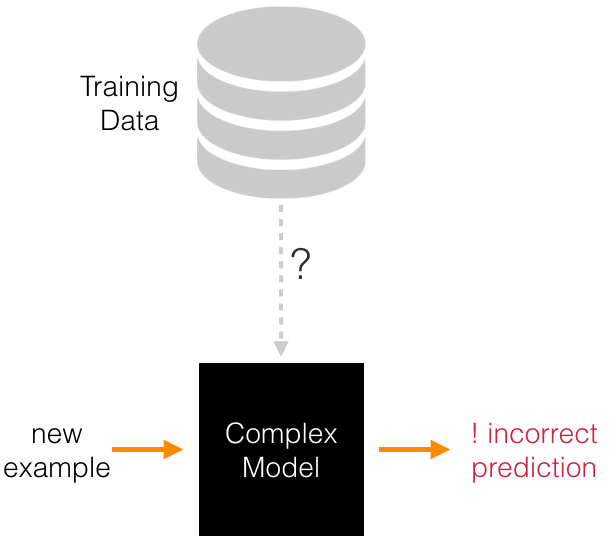
\includegraphics[width=0.35\columnwidth]{figures/teaser1.png}
    \hspace{2em}
    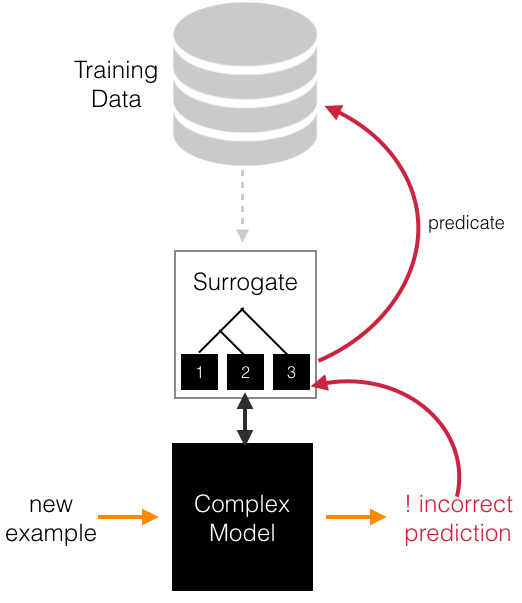
\includegraphics[width=0.35\columnwidth]{figures/teaser2.png}
    \caption{(Left) ML developers need to understand the relationship between training data and a model's predictions, i.e., how are similar points predicted in the training data. But effectively determining the size and range of this neighborhood is challenging in expressive models which can have very complex geometry. (Right) We propose an approximation technique that can represent a black-box model in terms of sub-models applied to feature-space partitions. The developer can quickly determine which data are related based on these partitions.}
    \label{fig:my_label}
\end{figure}

This problem is extremely challenging and the ML community has pursued two primary approaches: (1) use a simpler, more interpretable model (e.g., a decision tree) from the start, or (2) explain the behavior of a complex model using a simplified approximation~\cite{taylor2016alignment, lei2016rationalizing, ribeiro2016should}. Neither approach is perfect. 
Using a simpler model sacrifices prediction accuracy, which is a trade-off that many model applications are not willing to make.
An example of the second approach is to train a sparse linear model in the local neighborhood of a mispredicted point as a proxy to explain the characteristics (features) that caused the misprediction\cite{taylor2016alignment, lei2016rationalizing, ribeiro2016should}.
Although these approximations can identify salient features, they do not help identify the {\it training data} that led the model towards the misprediction.
Identifying this training data is increasingly important when debugging deep neural network models due to their heavy reliance on training data rather than feature engineering.
In addition, identifying training data can help developers differentiate between errors due to the model and errors due to training data.


%These approximations are effective because they can explain a prediction in terms of features of the input data (e.g., linear weights), but are these approximations also useful for debugging?
%However, these approximations only explain how a model predicts based on features, not what data led the model to predict in that way in the first place.
% We argue that the ML developers are concerned about what training data most influenced a prediction (i.e., if that data were not present in the training set would the prediction still have been wrong), as this allows them to differentiate between modeling errors and data errors.


Intuitively, the developer would like to isolate a subset of the training data that helps explain a misprediction. 
However, for most models, every training data point has some impact on the final result.
Thus, we simplify the problem to instead identify a {\it sub-partition} of the training data locally approximates the complex model for test points within this sub-partition.  


To this end, we present \sysfull (\sys).   \sys decomposes a complex model (e.g., a deep neural network) using a two-part {\it surrogate model}: a meta-model that partitions the training data, and a set of sub-models that approximate the patterns within each partition.
These sub-models can be arbitrarily complex in order to capture local patterns, however the meta-model is constrained to be a decision tree.
This formulation ensures that sub-models are accurate, while the partitions are interpretable as rules.
In contrast to existing model interpretation techniques that return locally relevant features, our approach returns the most informative neighborhood (partition).

Applying the trained surrogate model is very simple---if a test point is mispredicted, then we can identify the partition it belongs to and investigate that subset of the training data and its associated sub-model.
As our experiments show, the developer can tune the total number of sub-models and the depth of the decision tree in order to control the trade-off between the specificity of the partitions and how similar the surrogate model is to the complex model.
By identifying an entire partition, this approach will naturally identify the training points that likely led to the misprediction, as well as other training points that were irrelevant.   However, we assume that filtering the training data, which can often contain millions or trillions of data points, into a concise starting point for the developer to further explore the training data and more quickly identiy the problematic training data.

The rest of this short paper describes the \sys problem formulation, an algorithm sketch for training surrogate models, as well as an illustration of how \sys can be integrated in a visual model building interface.
Our experiments show that we can generate Fast, Approximated but Clear Explanations using \sys.
Furthermore, \ewu{NEED EXPERIMENT SUMMARY}
%We have applied our approach to control problems and find that it can improve 
%Our initial results have demonstrated that such an approach can improve convergence and stability in control problems.


\if{0}
This leads to our formalization of \emph{debuggability}.
Let $M$ be a model trained on a dataset of feature and label tuples $(x_i,y_i)$.
Suppose, M sees a new example $x'$ and predicts $y'$ causing a \emph{prediction anomaly} (i.e., incorrect prediction or unsafe output).
Debugability is a measure of how well can we isolate tuples in the training dataset that significantly contributed to the prediction $y'$.
Using this working definition, we can actually design algorithms that take in a black-box model and return a more debugable approximation.
In prior work, we have developed algorithms that can take a set of predictions from a model and infer a likely hierarchical structure~\cite{DBLP:journals/corr/KrishnanGLMPG16, Krishnan17}.
The basic idea is an iterative clustering algorithm that first initializes $k$ models, then assigns tuples to the model that best predicts it, then updates the $k$ models and repeats.
Once the k models are trained, we can then learn a meta-model to switch between them.
When a new example for prediction comes in, the meta-model first picks a sub-model, then the sub-model issues a prediction.
Our initial results have demonstrated that such an approach can improve convergence and stability in control problems.
\fi




























